\documentclass{article}%
\usepackage[a4paper, total={6in, 8in}]{geometry}

\usepackage[fleqn]{amsmath}
\usepackage{xcolor}
\usepackage{mathtools, nccmath}
\usepackage{algorithm}
\usepackage[noend]{algpseudocode}
\usepackage{graphicx}
\usepackage{listings}
\lstset{basicstyle=\ttfamily,
  showstringspaces=false,
  commentstyle=\color{red},
  keywordstyle=\color{blue}
}
\graphicspath{ {./images/}  }


\title{3-Dimensional Navier-Stokes in C++ Framework and Parallelization Techniques Comparison }
\date{2019\\ May}
\author{Christoph Neuhauser\\ Computer Science , Technical University of Munich 
\and Stefan Haas\\ Computer Science , Technical University of Munich
\and Kwok Ping Ng\\ Data Engineering and Analytics , Technical University of Munich}
\begin{document}
\maketitle

\section{Introduction}

After experiencing 2D Navier-Stokes Equation, Navier-Stokes Equation in 3D has been implemented in our group project.  C++ framework was replacing the traditional C programming. Then 3D calculation for velocity(u,v,w), force(F,G,H) ,pressure, residual and temperature has been reformed.  Due to increase in the complexity of arbitrary geometry in 3D, a new algorithm was implemented.

Our another goal was to elaborate how the CFD solver could be parallelized in a very efficient way. For this, we chose to compare a solver written in C++ with OpenMP (short: cpp solver), a solver using MPI for distributed-memory parallelism, a solver using CUDA on NVIDIA GPUs and a solver using OpenCL, which can be run on NVIDIA GPUs, Intel iGPUs and AMD GPUs. In the following section, we will descirbe the code and how to use it as well as compare these solvers regarding their best performance results, their scalability and their parallel efficiency.

\section{Code description}
\subsection{Code framwork}
The C++ Code is structured as follows. In the main directory is the main function where the main algorithm resides, which is basically the same algorithm like in the 2D CFD-Code. There also is the Defines.hpp file, which defines the floating-point precision as well as some used define statements for the use of indices.

Then there is the IO folder which holds everthing that has to do with input and output. Escpecially the VTK as well as the NetCDF writer and some classes to read and process different input formats for the geometry.

The importest part is the CdfSolver folder, where all solvers as well as the solver interface is. The interface defines the following methods:\pagebreak

\begin{lstlisting}[language=C++,frame=single]
void initialize(
    const std::string &scenarioName,
    LinearSystemSolverType linearSystemSolverType,
    bool shallWriteOutput, Real Re, Real Pr, Real omg, Real eps,
    int itermax, Real alpha, Real beta, Real dt, Real tau,
    Real GX, Real GY, Real GZ, bool useTemperature, Real T_h, Real T_c,
    int imax, int jmax, int kmax, Real dx, Real dy, Real dz,
    Real *U, Real *V, Real *W, Real *P, Real *T, uint32_t *Flag)
\end{lstlisting}
which copies the passed initial values of U, V, W, P, T and Flag to the internal representation of the solver.

\begin{lstlisting}[language=C++,frame=single]
void setBoundaryValues()
\end{lstlisting}
which sets the boundary condition values of U, V, W and T using the Flag array.

\begin{lstlisting}[language=C++,frame=single]
void setBoundaryValuesScenarioSpecific()
\end{lstlisting}
which sets special boundary conditions (typically something like inflow) specific to the different scenarios.

\begin{lstlisting}[language=C++,frame=single]
Real calculateDt()
\end{lstlisting}
which calculates the smallest possible (plus some safety margin) time step for the simulation at the current state.

\begin{lstlisting}[language=C++,frame=single]
void calculateTemperature()
\end{lstlisting}
which updates the temperature values (using an intermediate copy of the temperature from the last iteration).

\begin{lstlisting}[language=C++,frame=single]
void calculateFgh()
\end{lstlisting}
which computes the values in the helper array F, G and H necessary to compute the right-hand-side of the Pressure.

\begin{lstlisting}[language=C++,frame=single]
void calculateRs()
\end{lstlisting}
which computes the right-hand-side of the Pressure Poisson Equation (PPE).

\begin{lstlisting}[language=C++,frame=single]
void executeSorSolver()
\end{lstlisting}
which executes the SOR solver (successive over-relaxation) for solving the Pressure Poisson Equation (PPE).

\begin{lstlisting}[language=C++,frame=single]
void calculateUvw()
\end{lstlisting}
which updates the values in the arrays U, V and W.

\begin{lstlisting}[language=C++,frame=single]
void getDataForOutput(Real *U, Real *V, Real *W, Real *P, Real *T)
\end{lstlisting}
which copies the values of the internal representations of U, V, W, P and T to the specified arrays. This is necessary when outputting the simulation results at certain time intervals.

The CfdSolver directory also features classes to work with the flag array as well as to initiallise the arrays for the different variables.

Then there are the folders which have the solvers in them. Each solver has the same basic structure even though some have additional files and classes for different functions. Each solver has a file to manage the boundary values, the actuall CfdSolver class which mostly initiallizes variables and calls the function or kernels of the other files, the SOR solver file, where the SOR, Jacobi and/or the Gauss-Seidel solver are defined and finally the UVW file, which calculates everything what has to do with u,v or w, the temperature or the timestep.

\subsection{Building the code}
The program is compiled with cmake. To build it some packages have to installed (see README for more information how to install them on ubuntu) and the following commands have to be issued within the repository directory:
\begin{lstlisting}[language=bash,frame=single]
mkdir build
cd build
cmake ..
make
\end{lstlisting}

To use the different solvers some arguments have to be given to cmake. The following list shows these arguments:
\begin{itemize}
\item For MPI support: cmake .. -DUSE\_MPI=ON
\item For CUDA support: cmake .. -DUSE\_CUDA=ON
\item For OpenCL support: cmake .. -DUSE\_OPENCL=ON
\end{itemize}
These arguments can also be used together for the program to support multiple solvers at once.

\subsection{Running the program}
When executing the program multiple arguments can be passed on the command line. These arguments are shown in the following list as well as their respective valid values.
\begin{itemize}
\item scenario:
	\begin{itemize}
	\item driven\_cavity
	\item flow\_over\_step
	\item natural\_convection
	\item rayleigh\_benard\_convection\_8-2-1
	\item rayleigh\_benard\_convection\_8-2-2
	\item rayleigh\_benard\_convection\_8-2-4
	\item rayleigh\_benard\_convection\_2d
	\item single\_tower\item terrain\_1
	\end{itemize}
\item solver:
	\begin{itemize}
	\item cpp
	\item mpi
	\item cuda
	\item opencl
	\end{itemize}
\item outputformat:
	\begin{itemize}
	\item netcdf
	\item vtk (= vtk-binary)
	\item vtk-binary
	\item vtk-ascii
	\end{itemize}
\item output:
	\begin{itemize}
	\item true
	\item false (whether to write an output file)
	\end{itemize}
\item linsolver:
	\begin{itemize}
	\item jacobi
	\item sor
	\item gauss-seidel
	\end{itemize}
\item tracestreamlines:
	\begin{itemize}
	\item false
	\item true
	\end{itemize}
\item tracestreaklines:
	\begin{itemize}
	\item false
	\item true
	\end{itemize}
\item tracepathlines:
	\begin{itemize}
	\item false
	\item true
	\end{itemize}
\item numparticles:
	\begin{itemize}
	\item any positive integer number
	\end{itemize}
\item numproc
	\begin{itemize}
	\item Must be used with the MPI solver. Specifys the number of processes in x, y and z direction and must match the total number of MPI processes.
	\item possible values: positive integer positive integer positive integer
	\item example: --numproc = 2 2 2
	\end{itemize}
\item blocksize
	\begin{itemize}
	\item Can be used with the CUDA or the OpenCL solver. Specifys the block size in x, y and z direction.
	\item possible values: positive integer positive integer positive integer
	\item example: --blocksize = 4 4 4
	\end{itemize}
\item platformid
	\begin{itemize}
	\item Can be used with the OpenCL solver. Specifys the ID of the OpenCL platform to use. If the ID is not specified, it is set to zero. Which platform corresponds to which ID can be found outwith the command line tool 'clinfo'.
	\item possible values: integer
	\end{itemize}
\end{itemize}

\noindent The standard values for the arguments are:
\begin{itemize}
\item scenario: driven\_cavity
\item solver: cpp
\item outputformat: vtk
\item outputformat: true
\item linsolver: jacobi
\item tracestreamlines: false
\item tracestreaklines: false
\item tracepathlines: false
\item numparticles: 1000
\item blocksize: 8 8 4
\item platformid: 0
\end{itemize}

Here are some examples on how the code can be run:
\begin{lstlisting}[language=bash, frame=single]
./cfd3d --scenario driven_cavity --solver cpp
mpirun -np 8 ./cfd3d --solver mpi --numproc 2 2 2
./cfd3d --scenario driven_cavity --solver cuda
\end{lstlisting}





\section{3D incompressible Navier-Stokes equation}
Non-stationary incompressible viscous fluid flow is described in 3-dimensional Navier-Stokes Equation. The analysis was carried out in Cartesian coordinates. The quantities are computed as u,v,w and F,G,H as x,y,z directions.

\subsection{3D Momentum equations}
\begin{equation}
\frac{\partial u}{\partial t} + \frac{\partial p}{\partial x} = 
\frac{1}{Re} \left( \frac{\partial^2 u}{\partial x^2} + \frac{\partial^2 u}{\partial y^2} + \frac{\partial^2 u}{\partial z^2} \right) - 
\frac{\partial(u^2)}{\partial x} -\frac{\partial (uv)}{\partial y} - 
\frac{\partial (uw)}{\partial z} +
g_x 
\end{equation}

\begin{equation}
\frac{\partial v}{\partial t} + \frac{\partial p}{\partial y} = 
\frac{1}{Re} \left( \frac{\partial^2 v}{\partial x^2} + \frac{\partial^2 v}{\partial y^2} + \frac{\partial^2 v}{\partial z^2} \right) - 
\frac{\partial(uv)}{\partial x} -\frac{\partial (v^2)}{\partial y} - 
\frac{\partial (vw)}{\partial z} +
g_y
\end{equation}

\begin{equation}
\frac{\partial w}{\partial t} + \frac{\partial p}{\partial z} = 
\frac{1}{Re} \left( \frac{\partial^2 w}{\partial x^2} + \frac{\partial^2 w}{\partial y^2} + \frac{\partial^2 w}{\partial z^2} \right) - 
\frac{\partial(uw)}{\partial x} -\frac{\partial (vw)}{\partial y} - 
\frac{\partial (w^2)}{\partial z} +
g_z
\end{equation}

\subsection{3D Continuity equation}
\begin{equation}
\frac{\partial u}{\partial x} + \frac{\partial v}{\partial y} + \frac{\partial w}{\partial z} = 0
\end{equation}

\subsection{Force F and velocity u calculation in x direction}
Velocity w is essentially considered into the calculation then, the discretization for derivatives of u,v and w has to be with respect to directions x,y and z respectively.\\
\\
F:
\begin{equation}
\begin{split}
F_{i,j,k} =
u_{i,j,k} & + \delta t \Bigl(
\frac{1}{Re} \left( \left[\frac{\partial^2 u}{\partial x^2}\right]_{i,j,k} + \left[\frac{\partial^2 u}{\partial y^2}\right]_{i,j,k} + \left[\frac{\partial^2 u}{\partial z^2}\right]_{i,j,k} \right) - 
\left[\frac{\partial(u^2)}{\partial x}\right]_{i,j,k} -\left[\frac{\partial (uv)}{\partial y}\right]_{i,j,k} - 
\left[\frac{\partial (uw)}{\partial z}\right]_{i,j,k}\\
& + {g_x} - \frac{\beta}{2} \left( T^{(n+1)}_{i,j,k} + T^{(n+1)}_{i+1,j,k} \right) g_x \Bigr)\\
& i = 1,\ldots,imax-1; \quad j = 1,\ldots,jmax; \quad k = 1,\ldots,kmax
\end{split}
\end{equation}
u:\\
\begin{equation}
\begin{split}
u^{(n+1)}_{i,j,k} = & F^{(n)}_{i,j,k} - \frac{\delta t}{\delta x}\left(p^{(n+1)}_{i+1,j,k} - p^{(n+1)}_{i,j,k}\right)\\
& i = 1,\ldots,imax-1; \quad j = 1,\ldots,jmax; \quad k = 1,\ldots,kmax
\end{split}
\end{equation}

\subsection{Discretization for F}
The midpoints of 3 directions will be towards to evaluate the derivative of u,v and w:\\
\begin{equation}
\left[\frac{\partial^2 u}{\partial x^2}\right]_{i,j,k} =
\frac{u_{i+1,j,k} - 2u_{i,j,k} + u_{i-1,j,k}}{(\delta x)^2}
\end{equation}

\begin{equation}
\left[\frac{\partial^2 u}{\partial y^2}\right]_{i,j,k} =
\frac{u_{i,j+1,k} - 2u_{i,j,k} + u_{i,j-1,k}}{(\delta y)^2}
\end{equation}

\begin{equation}
\left[\frac{\partial^2 u}{\partial z^2}\right]_{i,j,k} =
\frac{u_{i,j,k+1} - 2u_{i,j,k} + u_{i,j,k-1}}{(\delta z)^2}
\end{equation}

\begin{equation}
\begin{split}
\left[\frac{\partial(u^2)}{\partial x}\right]_{i,j,k} = &
\frac{1}{\delta x}
\left(
	\left(\frac{u_{i,j,k}+u_{i+1,j,k}}{2}\right)^2 -
	\left(\frac{u_{i-1,j,k}+u_{i,j,k}}{2}\right)^2
\right) + \\
& \frac{\gamma}{\delta x}
\left(
	\frac{|u_{i,j,k}+u_{i+1,j,k}|}{2} \frac{(u_{i,j,k}-u_{i+1,j,k})}{2} -
	\frac{|u_{i-1,j,k}+u_{i,j,k}|}{2} \frac{(u_{i-1,j,k}-u_{i,j,k})}{2}
\right)
\end{split}
\end{equation}

\begin{equation}
\begin{split}
\left[\frac{\partial(uv)}{\partial y}\right]_{i,j,k} = &
\frac{1}{\delta y}
\left(
	\frac{(v_{i,j,k}+v_{i+1,j,k})}{2} \frac{(u_{i,j,k}+u_{i,j+1,k})}{2} -
	\frac{(v_{i,j-1,k}+v_{i+1,j-1,k})}{2} \frac{(u_{i,j-1,k}+u_{i,j,k})}{2}
\right) + \\
& \frac{\gamma}{\delta y}
\left(
	\frac{|v_{i,j,k}+v_{i+1,j,k}|}{2} \frac{(u_{i,j,k}-u_{i,j+1,k})}{2} -
	\frac{|v_{i,j-1,k}+v_{i+1,j-1,k}|}{2} \frac{(u_{i,j-1,k}-u_{i,j,k})}{2}
\right)
\end{split}
\end{equation}

\begin{equation}
\begin{split}
\left[\frac{\partial(uw)}{\partial z}\right]_{i,j,k} = &
\frac{1}{\delta z}
\left(
	\frac{(w_{i,j,k}+w_{i+1,j,k})}{2} \frac{(u_{i,j,k}+u_{i,j,k+1})}{2} -
	\frac{(w_{i,j,k-1}+w_{i+1,j,k-1})}{2} \frac{(u_{i,j,k-1}+u_{i,j,k})}{2}
\right) + \\
& \frac{\gamma}{\delta z}
\left(
	\frac{|w_{i,j,k}+w_{i+1,j,k}|}{2} \frac{(u_{i,j,k}-u_{i,j,k+1})}{2} -
	\frac{|w_{i,j,k-1}+w_{i+1,j,k-1}|}{2} \frac{(u_{i,j,k-1}-u_{i,j,k})}{2}
\right)
\end{split}
\end{equation}
\subsection{Energy equation and Discretization}
The energy equation in 3D and its discretization are easy to compute:\\
\\
Energy Equation:\\
\begin{equation}
T^{(n+1)}_{i,j,k} = T^{(n)}_{i,j,k} +  \delta t \left(
\frac{1}{Re} \frac{1}{Pr} \left( \left[\frac{\partial^2 T}{\partial x^2}\right]_{i,j,k} + \left[\frac{\partial^2 T}{\partial y^2}\right]_{i,j,k} + \left[\frac{\partial^2 T}{\partial z^2}\right]_{i,j,k} \right) 
- 
\left[\frac{\partial(uT)}{\partial x}\right]_{i,j,k} -\left[\frac{\partial (vT)}{\partial y}\right]_{i,j,k} - 
\left[\frac{\partial (wT)}{\partial z}\right]_{i,j,k}
\right)
\end{equation}
Discretization:\\
\begin{equation}
\left[\frac{\partial^2 T}{\partial x^2}\right]_{i,j,k} =
\frac{T_{i+1,j,k} - 2T_{i,j,k} + T_{i-1,j,k}}{(\delta x)^2}
\end{equation}

\begin{equation}
\begin{split}
\left[\frac{\partial(uT)}{\partial x}\right]_{i,j,k} = &
\frac{1}{\delta x}
\left(
	u_{i,j,k} \frac{T_{i,j,k}+T_{i+1,j,k}}{2} -
	u_{i-1,j,k} \frac{T_{i-1,j,k}+T_{i,j,k}}{2}
\right) + \\
& \frac{\gamma}{\delta x}
\left(
	|u_{i,j,k}| \frac{T_{i,j,k}-T_{i+1,j,k}}{2} -
	|u_{i-1,j,k}| \frac{T_{i-1,j,k}-T_{i,j,k}}{2}
\right)
\end{split}
\end{equation}
\subsection{SOR Solver}
Pressure:\\
\begin{equation}
\begin{split}
p^{it+1}_{i,j,k} = & (1 - \omega) p^{it}_{i,j,k} + \frac{\omega}{2 (\frac{1}{(\delta x)^2} + \frac{1}{(\delta y)^2} + \frac{1}{(\delta z)^2})} \left( \frac{p^{it}_{i+1,j,k} + p^{it+1}_{i-1,j,k}}{(\delta x)^2} + \frac{p^{it}_{i,j+1,k} + p^{it+1}_{i,j-1,k}}{(\delta y)^2} + \frac{p^{it}_{i,j,k+1} + p^{it+1}_{i,j,k-1}}{(\delta z)^2} - rs_{i,j,k} \right)\\
& it = 1,\ldots,itmax; \quad i = 1,\ldots,imax; \quad j = 1,\ldots,jmax; \quad k = 1,\ldots,kmax
\end{split}
\end{equation}
Residual:\\
\begin{equation}
\begin{split}
res := & \left( \sum_{i=1}^{imax} \sum_{j=1}^{jmax} \sum_{k=1}^{kmax} \left( \frac{p_{i+1,j,k} - 2 p_{i,j,k} + p_{i-1,j,k}}{(\delta x)^2} + \frac{p_{i,j+1,k} - 2 p_{i,j,k} + p_{i,j-1,k}}{(\delta y)^2} + \frac{p_{i,j,k+1} - 2 p_{i,j,k} + p_{i,j,k-1}}{(\delta z)^2} \right. \right. \\
& \left. \left. - rs_{i,j,k} \right)^2 / (imax \cdot jmax \cdot kmax) \right)^{1/2}
\end{split}
\end{equation}
\section{Boundary Conditions}
\subsection{No Slip} 
Under the no-slip conditions, zero velocities at boundary. So we can set it to zero lying right on the boundary. Moreover, the boundary value zero is achieved by averaging the values on both sides of the boundary. For example, left wall case: $u_{0,j,k}$ = 0 ,$v_{0,j,k}$ = -$v_{1,j,k}$, $w_{0,j,k}$ = -$w_{1,j,k}$.
\subsection{Free Slip} 
It is the case when fluid flow freely parallel to the boundary but cannot across the boundary. In 3D cases, the fluid freely flow along two dimension but cannot across remaining direction. For example, the velocity u of left wall which is normal(perpendicular) to the wall is 0. Its boundary condition is to set as $u_{0,j,k}$ = 0. And other boundary conditions to set $v_{0,j,k}$ = $v_{1,j,k}$, $w_{0,j,k}$ = $w_{1,j,k}$. See Figure 1 below.

\begin{figure}[h]
    \centering
    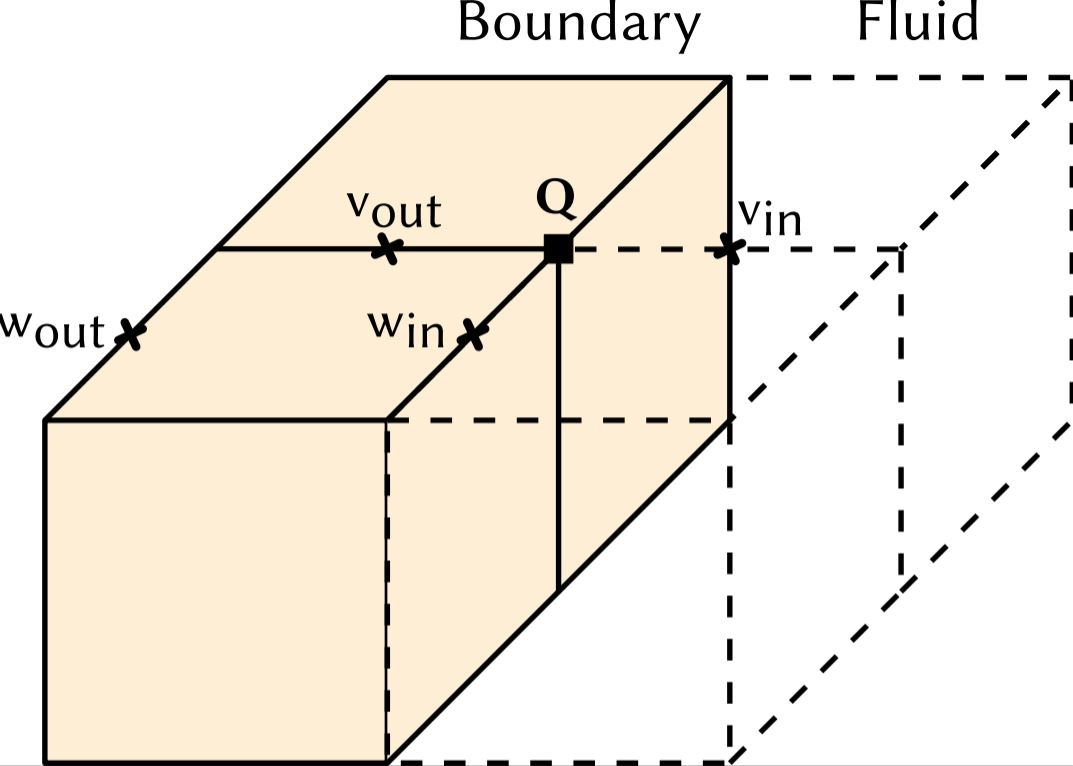
\includegraphics[width=6cm, height=5cm]{freeslip}
    \caption{Free-slip}
    \label{fig:mesh1}
\end{figure}

\subsection{Outflow}
the normal velocity derivatives are set to 0 at boundary. So the total velocity does not change in the direction normal to the boundary. The values of velocities at boundary can be set equal to the neighbouring velocities inside the region. For example,left wall case: $u_{0,j,k}$ = $u_{1,j,k}$ ,$v_{0,j,k}$ = $v_{1,j,k}$, $w_{0,j,k}$ = $w_{1,j,k}$
\subsection{Boundary conditions for pressure and temperature}
The boundary conditions for the pressure derived from momentum equation, resulting in discrete Neumann conditions. The boundary conditions for temperature derived from energy equation, resulting in discrete Dirichlet Condition for cold wall and hot wall separately. For example, left wall case: $P_{0,j,k}$ = $P_{1,j,k}$.  $T_{0,j,k}$ = $2*T_c/T_h$ – $T_{1,j,k}$.

\section{Performance}
\subsection{CUDA}
First of all, on consumer hardware, the CUDA solver and the OpenCL solver had considerable advantages over the CPU solvers. They can be seen in figure~\ref{fig:platforms} which where run on on a NVIDIA GeForce GTX 1070, a 6-core Intel Core i7-8700 and on a 28-core Intel Xeon E5-2697 from the Linux Cluster of the LRZ. Graphics cards offer a much higher number of cores available for applications to utilize compared to similar prized-processors. However, GPUs execute workloads in a SIMD-fashion in lockstep, which means that a thread warp (that usually consists of 32 or 64 individual threads) would need to go the same route in the code without any diverging branches to reach the maximum possible performance. Furthermore, another problem is that especially NVIDIA limits their double-precision performance on consumer-level graphics cards to create an additional sales rationale for their high-priced workstation cards.

In theory, according to \cite{cuda-guide}, the throughput of arithmetic double-precision floating point instructions on the GTX 1070 would be 1 : 32. However, the CUDA solver proved to be only approximately 48\text{\%} slower in our test case for double-precision floating points values compared to single-precision floating point values, which can be seen in figure~\ref{fig:platforms}. This can be probably attributed to the application being memory throughput limited for floating point operations rather than being limited by the throughput of arithmetic instructions.

On modern CPU architectures, the floating point units (FPUs) don’t offer separate modules for single-precision and double-precision instructions anymore. Thus, as expected, the CPU solvers were only approximately 2\text{\%} slower for double-precision floating-point numbers compared to single-precision floating-point numbers. The slight reduce in performance can probably also be attributed to the higher memory throughput of 64-bit wide double-precision floating-point numbers.

\subsection{MPI}
When comparing the scalability of the solvers, it is of course clear that the MPI solver offers the best scalability, as a memory-distributed program can be scaled to an arbitrary amount of cores. The weakness of the MPI solver comes into play when comparing it to a shared-memory implementation of the CFD solver on systems with a moderate number of cores. On our 6-core test system, the MPI solver was approximately 35\text{\%} slower than the OpenMP solver. Figure~\ref{fig:platforms} shows this difference. This is of course due to the communication overhead for the MPI solver. The advantage of MPI comes into play when utilizing multiple nodes of a cluster at once with distributed memory.
When using two nodes and 56 cores, the MPI solver (with a domain decomposition of 7x4x2) gave by far the best performance results of all CPU solvers, but the CUDA solver still was 85\text{\%} faster on the NVIDIA GeForce GTX 1070 even when using double-precision performance. There are probably two reasons for that. First of all, we used strong scaling with a fixed global problem size of 80x20x10 cells. It is of course comprehensible that the overhead for communication becomes really large for this high number of processes and a small local domain size. Secondly, the CUDA solver is able to very efficiently utilize the SIMD functionality of the GPU to provide a really large number of threads accessing very fast shared GDDR5 memory without hardly any communication overhead.

\begin{figure}[htb]
\centering
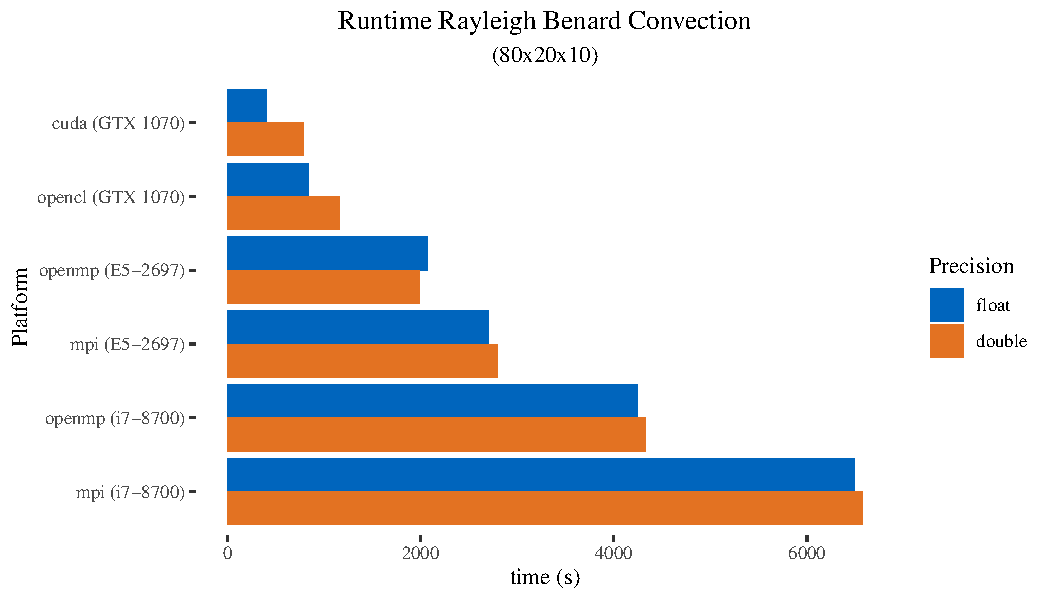
\includegraphics[width=1\linewidth]{../tests/graphs/runtime_rayleigh_benard_convection_8-2-1_platforms.pdf}
\caption{Write caption here.}
\label{fig:platforms}
\end{figure}

\subsection{SOR and alternatives}
When parallelizing the CFD solver, it is also necessary to parallelize the solver used for the linear system of equations of the Pressure Poisson Equation (PPE).

For the parallel solvers, we decided to implement and compare a Jacobi, Gauss-Seidel (GS) and successive over-relaxation (SOR) solver. Each of the solvers has its own advantages and disadvantages.

Jacobi is the solver to converge slowest (measured by the number of iterations, not the runtime on multiple cores). However, its greatest advantage is that it can be easily parallelized, as it has no data dependencies within one iteration.

Gauss-Seidel converges in less iterations than Jacobi, but is harder to parallelize. The vanilla SOR algorithm without any adaptions generally cannot run in parallel. Thus, Gauss-Seidel only has an advantage over Jacobi when using a low number of cores. We tested the parallel SOR solver by Cunha and Hopkins \cite{parallel-sor}, but for sparse system matrices like in our case, the sequential update step in the end of the algorithm quickly becomes limiting for a high number of cores due to Amdahl’s law.

SOR is an algorithm based on Gauss-Seidel that couples the algorithm with an over-relaxation factor that can increase the convergence speed. In our program, we tested multiple values, and got the best results for an over-relaxation factor of 1.5. In our tests, which can be seen in figure~\ref{fig:solver}, Gauss-Seidel was faster than SOR, which we didn't expect. Again, SOR suffers from the same weakness as Gauss-Seidel that it can’t be parallelized easily. Thus, again, for a high number of cores, the Jacobi solver was able to beat the SOR solver.

Another method for solving a system of linear equations mentioned less often is the Jacobi over-relaxation (JOR), which transfers the principle of SOR to the Jacobi solver. However, for over-relaxation factors greater than 1, the solution would not converge. Thus, we rejected the JOR solver, as it can only increase convergence speed for a factor larger than 1. In the literature, we couldn’t find any other source having success with JOR coupled with a factor greater than 1.

Taking all factors mentioned above into account, we decided to select the Jacobi solver as the standard solver in our program, as it converges considerably faster in the same time compared to the SOR solver for a high number of cores. In figure~\ref{fig:solver} it can be seen, that the difference between the solver when using MPI is really small, since all solvers are parallelised. In the case of Openmp our tests show that our decision to use Jacobi was correct.

\begin{figure}[htb]
\centering
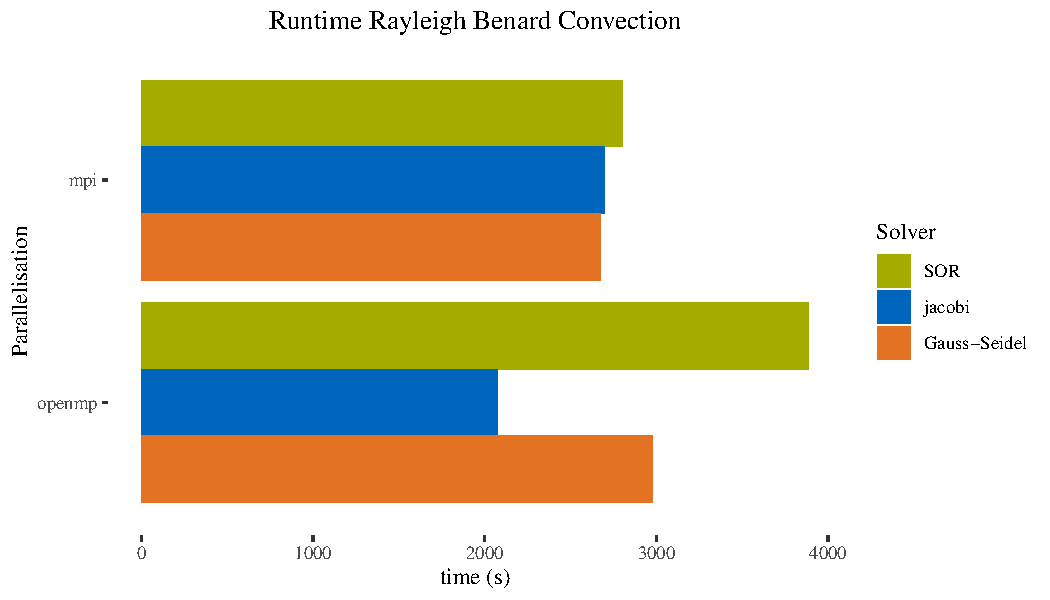
\includegraphics[width=1\linewidth]{../tests/graphs/runtime_rayleigh_benard_convection_8-2-1_solver.pdf}
\caption{Write caption here.}
\label{fig:solver}
\end{figure}


\subsection{Speedup}
After we chose the best solver we tested the performance when using a different number of cores. These tests were run on the Linux Cluster of the LRZ, where we used one node with a Intel Xeon E5-2697 for the speedup tests with OpenMP and up to two nodes with the same processor for the speedup tests with MPI.

The results of the tests with OpenMP can be seen in figure~\ref{fig:speedup_openmp}. The speedup is exactly as we expected. At the beginning the performance scales very good while the speedup at the end degrades. At 28 cores the speedup is approximately 14.

To test the MPI implementation we used one node for the first test. The reason we used 27 out of the 28 cores is that the domain could be split better with this amount of mpi processes, since the domain can be split in 3x3x3 parts, whereas with 28 processes it would be split into 7x2x2 part. We also tested both variants and the version with 27 processes was faster. With 27 cores the speedup is around ten which is not as good as with OpenMP, but when using two nodes with 56 cores altogether, the performance scales almost linearly with an speedup of approximately 19, even though the domain is split in 7x4x2 part, which is not optimal.


\begin{figure}[htb]
\centering
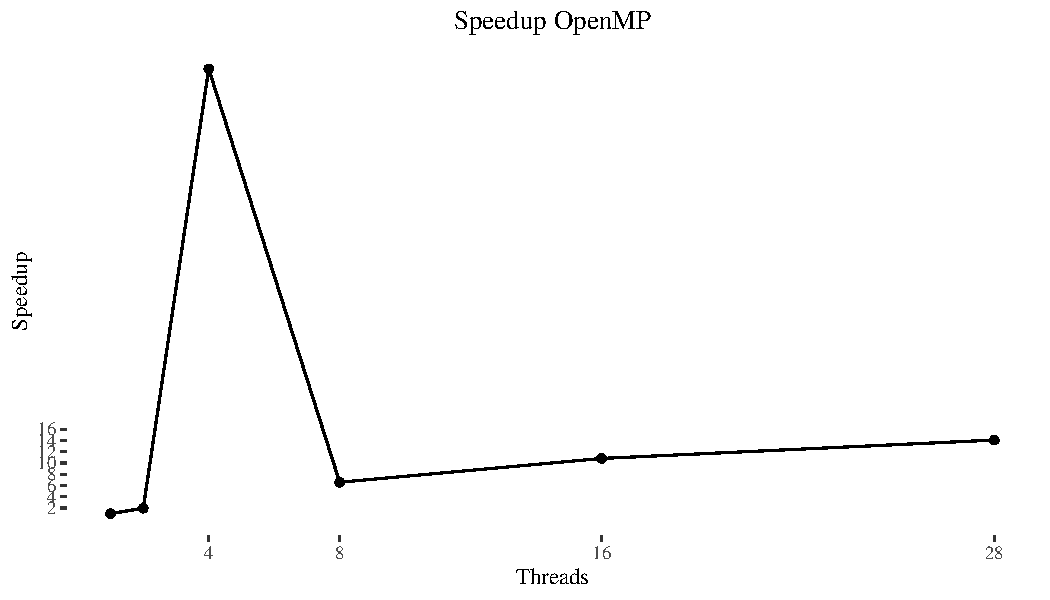
\includegraphics[width=1\linewidth]{../tests/graphs/speedup_OpenMP_double.pdf}
\caption{Write caption here.}
\label{fig:speedup_openmp}
\end{figure}

\begin{figure}[htb]
\centering
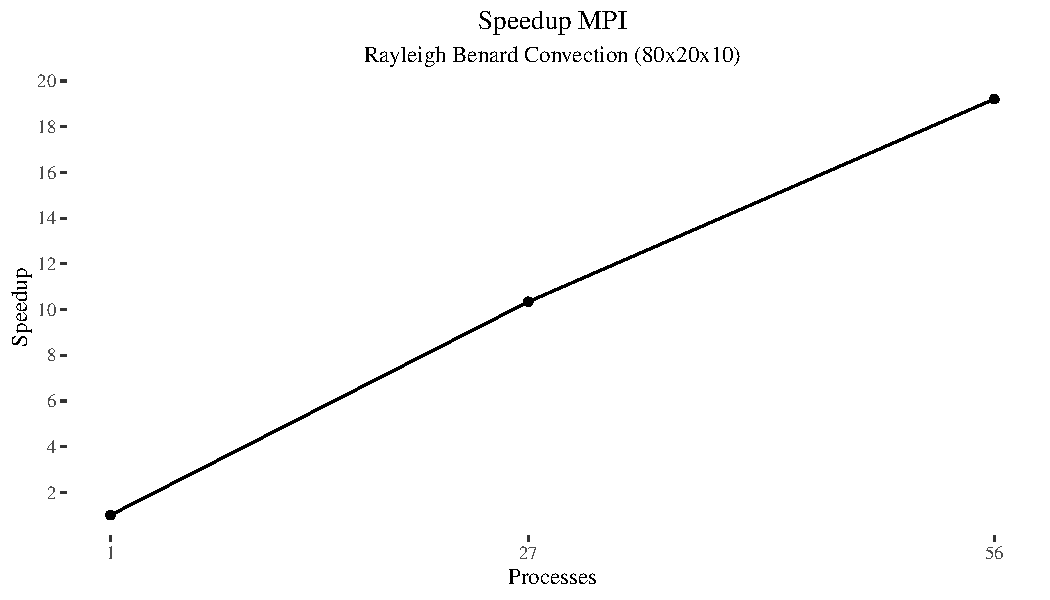
\includegraphics[width=1\linewidth]{../tests/graphs/speedup_MPI.pdf}
\caption{Write caption here.}
\label{fig:speedup_MPI}
\end{figure}


\section{Arbitrary Geometries}
\subsection{u,v,w}
Unlike the 2D cases which is necessarily to set the arbitrary geometries of velocities for 8 directions(4 lines + 4 corners of a square), there are total 26 directions (12 lines, 8 corners and 6 faces of a cube) to be set. Then setting it in 3D brought difficulties if we used the method from ws2.  Therefore, we designed a new algorithm to set arbitrary geometries.

We observed that we could set velocity to zero lying right on the boundary. Moreover, the boundary value zero was achieved by averaging the values on both sides of the boundary. It was the similar case to set no-slip boundary condition on walls.  We set u,v and w separately . The flag of direction was checked if the velocity was lying on. If yes, the velocity was set to zero. Then an indicator was inserted that this velocity was not changed anymore. Otherwise, the velocity was set to equal to the negative of the neighbouring velocity.  For example, here is pseudo code of the arbitrary geometry setting of u on left wall.

\begin{algorithm}
\caption{Algorithm on left boundary}\label{euclid}
\begin{algorithmic}
\For{over i,j,k}
	\State $a\gets 0$
	\State $b\gets 0$ 
	\If {Flag is not fluid}
    	\If {Left flag is obstacle}
    		\State $u_{i-1,j,k}\gets 0$
    		\State $a\gets 1$
    	\EndIf
    	\If {Up flag is obstacle}
    		\If {$a == 0$}
    			\State $u_{i-1,j,k}\gets -u_{i-1,j+1,k}$
    			\State $b\gets 1$
    		\EndIf	
    	\EndIf
    	\If {Down flag is obstacle}
    		\If {$a == 0$}
    			\State $u_{i-1,j,k}\gets -u_{i-1,j-1,k}$
    			\State $b\gets 1$
    		\EndIf	
    	\EndIf 
    	\If {Back flag is obstacle}
    		\If {$a == 0$ and $b==0$}
    			\State $u_{i-1,j,k}\gets -u_{i-1,j,k-1}$
    			\State $b\gets 1$
    		\EndIf	
    	\EndIf    	   	
    	\If {Front flag is obstacle}
    		\If {$a == 0$ and $b==0$}
    			\State $u_{i-1,j,k}\gets -u_{i-1,j,k+1}$
    			\State $b\gets 1$
    		\EndIf	
    	\EndIf       	
\EndIf
\EndFor
\end{algorithmic}
\end{algorithm}

\subsection{Pressure and Temperature}
Setting the arbitrary geometry of pressure and temperature are using the same methodology. As the pressure and temperature at the direction is the average of the 6 faces involved, for example, $B\_URF$(up, right and front)’s pressure $P_{ijk} = (P_{i+1jk} + P_{ij+1k} + P_{ijk+1})/3$. So each flag of direction is checked and accumulated .  To sum up the pressure/temperature and take the average of them. 

\begin{algorithm}
\caption{Algorithm on Pressure}\label{euclid}
\begin{algorithmic}
\For{over i,j,k}
	\State $numDirectFlag\gets 0$
	\State $P\_temp\gets 0$
	\If {Flag is not fluid}
    	\If {Left flag is obstacle}
    		\State $P\_temp += P_{i+1,j,k}$
    		\State $numDirectFlag++$
    	\EndIf
    \State{...}	    	
    \State $P_{i,j,k}= P_temp / numDirectFlag$
\EndIf
\EndFor
\end{algorithmic}
\end{algorithm}



\begin{thebibliography}{999}

\bibitem{lamport94}
Nvidia,https://docs.nvidia.com/cuda/cuda-c-programming-guide/index.html\text{\#}arithmetic-instructions,5.4.1. Arithmetic Instructions
\bibitem{lamport94}
Rudnei Dias da Cunha, Tim Hopkins: “Parallel Overrelaxation Algorithms for Systems of Linear Equations” (1991)
\end{thebibliography}

\end{document}